% This file was created with matplot2tikz v0.4.0.
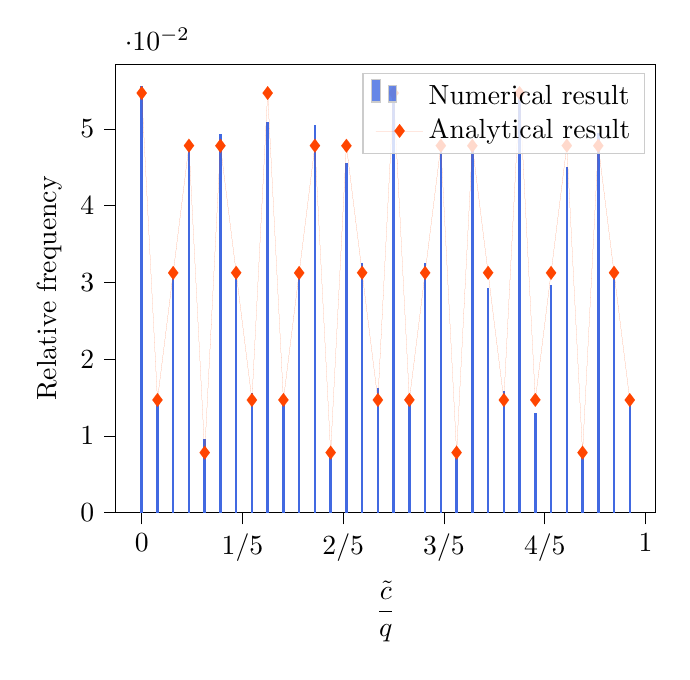
\begin{tikzpicture}

\definecolor{darkgray176}{RGB}{176,176,176}
\definecolor{lightgray204}{RGB}{204,204,204}
\definecolor{orangered}{RGB}{255,69,0}
\definecolor{royalblue}{RGB}{65,105,225}

\begin{axis}[
legend cell align={left},
legend style={fill opacity=0.8, draw opacity=1, text opacity=1, draw=lightgray204},
tick align=outside,
tick pos=left,
x grid style={darkgray176},
xlabel={\(\displaystyle \frac{\tilde{c}}{q}\)},
xmin=-0.0511875, xmax=1.0199375,
xtick style={color=black},
xtick={-0.2,0,0.2,0.4,0.6,0.8,1,1.2},
xticklabels={
  \(\displaystyle -1/5\),
  \(\displaystyle 0\),
  \(\displaystyle 1/5\),
  \(\displaystyle 2/5\),
  \(\displaystyle 3/5\),
  \(\displaystyle 4/5\),
  \(\displaystyle 1\),
  \(\displaystyle 6/5\)
},
y grid style={darkgray176},
ylabel={Relative frequency},
ymin=0, ymax=0.058447265625,
ytick style={color=black}
]
\draw[draw=none,fill=royalblue] (axis cs:-0.0025,0) rectangle (axis cs:0.0025,0.0556640625);
\addlegendimage{ybar,ybar legend,draw=none,fill=royalblue}
\addlegendentry{Numerical result}

\draw[draw=none,fill=royalblue] (axis cs:0.02875,0) rectangle (axis cs:0.03375,0.0150146484375);
\draw[draw=none,fill=royalblue] (axis cs:0.06,0) rectangle (axis cs:0.065,0.0306396484375);
\draw[draw=none,fill=royalblue] (axis cs:0.09125,0) rectangle (axis cs:0.09625,0.04827880859375);
\draw[draw=none,fill=royalblue] (axis cs:0.1225,0) rectangle (axis cs:0.1275,0.00958251953125);
\draw[draw=none,fill=royalblue] (axis cs:0.15375,0) rectangle (axis cs:0.15875,0.04937744140625);
\draw[draw=none,fill=royalblue] (axis cs:0.185,0) rectangle (axis cs:0.19,0.03118896484375);
\draw[draw=none,fill=royalblue] (axis cs:0.21625,0) rectangle (axis cs:0.22125,0.01556396484375);
\draw[draw=none,fill=royalblue] (axis cs:0.2475,0) rectangle (axis cs:0.2525,0.05096435546875);
\draw[draw=none,fill=royalblue] (axis cs:0.27875,0) rectangle (axis cs:0.28375,0.014892578125);
\draw[draw=none,fill=royalblue] (axis cs:0.31,0) rectangle (axis cs:0.315,0.03125);
\draw[draw=none,fill=royalblue] (axis cs:0.34125,0) rectangle (axis cs:0.34625,0.050537109375);
\draw[draw=none,fill=royalblue] (axis cs:0.3725,0) rectangle (axis cs:0.3775,0.00732421875);
\draw[draw=none,fill=royalblue] (axis cs:0.40375,0) rectangle (axis cs:0.40875,0.0455322265625);
\draw[draw=none,fill=royalblue] (axis cs:0.435,0) rectangle (axis cs:0.44,0.032470703125);
\draw[draw=none,fill=royalblue] (axis cs:0.46625,0) rectangle (axis cs:0.47125,0.01617431640625);
\draw[draw=none,fill=royalblue] (axis cs:0.4975,0) rectangle (axis cs:0.5025,0.05511474609375);
\draw[draw=none,fill=royalblue] (axis cs:0.52875,0) rectangle (axis cs:0.53375,0.014892578125);
\draw[draw=none,fill=royalblue] (axis cs:0.56,0) rectangle (axis cs:0.565,0.0325927734375);
\draw[draw=none,fill=royalblue] (axis cs:0.59125,0) rectangle (axis cs:0.59625,0.0478515625);
\draw[draw=none,fill=royalblue] (axis cs:0.6225,0) rectangle (axis cs:0.6275,0.007080078125);
\draw[draw=none,fill=royalblue] (axis cs:0.65375,0) rectangle (axis cs:0.65875,0.04815673828125);
\draw[draw=none,fill=royalblue] (axis cs:0.685,0) rectangle (axis cs:0.69,0.02923583984375);
\draw[draw=none,fill=royalblue] (axis cs:0.71625,0) rectangle (axis cs:0.72125,0.01580810546875);
\draw[draw=none,fill=royalblue] (axis cs:0.7475,0) rectangle (axis cs:0.7525,0.0548095703125);
\draw[draw=none,fill=royalblue] (axis cs:0.77875,0) rectangle (axis cs:0.78375,0.01300048828125);
\draw[draw=none,fill=royalblue] (axis cs:0.81,0) rectangle (axis cs:0.815,0.02960205078125);
\draw[draw=none,fill=royalblue] (axis cs:0.84125,0) rectangle (axis cs:0.84625,0.04498291015625);
\draw[draw=none,fill=royalblue] (axis cs:0.8725,0) rectangle (axis cs:0.8775,0.00762939453125);
\draw[draw=none,fill=royalblue] (axis cs:0.90375,0) rectangle (axis cs:0.90875,0.0494384765625);
\draw[draw=none,fill=royalblue] (axis cs:0.935,0) rectangle (axis cs:0.94,0.03131103515625);
\draw[draw=none,fill=royalblue] (axis cs:0.96625,0) rectangle (axis cs:0.97125,0.0140380859375);
\addplot [line width=0.0004pt, orangered, opacity=1, mark=diamond*, mark size=2.5, mark options={solid}]
table {%
3.125e-06 0.0546874981928215
0.031253125 0.0146836942229451
0.062503125 0.0312407961155092
0.093753125 0.0478293220353282
0.125003125 0.00781250180717853
0.156253125 0.0478163057770549
0.187503125 0.0312592038844907
0.218753125 0.0146706779646719
0.250003125 0.0546874981928215
0.281253125 0.0146836942229452
0.312503125 0.0312407961155092
0.343753125 0.0478293220353282
0.375003125 0.00781250180717847
0.406253125 0.0478163057770549
0.437503125 0.0312592038844907
0.468753125 0.0146706779646718
0.500003125 0.0546874981928215
0.531253125 0.014683694222945
0.562503125 0.0312407961155094
0.593753125 0.0478293220353282
0.625003125 0.00781250180717847
0.656253125 0.0478163057770549
0.687503125 0.0312592038844908
0.718753125 0.0146706779646717
0.750003125 0.0546874981928215
0.781253125 0.014683694222945
0.812503125 0.0312407961155094
0.843753125 0.0478293220353282
0.875003125 0.00781250180717847
0.906253125 0.0478163057770549
0.937503125 0.0312592038844908
0.968753125 0.0146706779646717
};
\addlegendentry{Analytical result}
\end{axis}

\end{tikzpicture}
